% !TeX program = pdfLaTeX
\documentclass[smallextended]{svjour3}       % onecolumn (second format)
%\documentclass[twocolumn]{svjour3}          % twocolumn
%
\smartqed  % flush right qed marks, e.g. at end of proof
%
\usepackage{amsmath}
\usepackage{graphicx}
\usepackage[utf8]{inputenc}

\usepackage[hyphens]{url} % not crucial - just used below for the URL
\usepackage{hyperref}
\providecommand{\tightlist}{%
  \setlength{\itemsep}{0pt}\setlength{\parskip}{0pt}}

%
% \usepackage{mathptmx}      % use Times fonts if available on your TeX system
%
% insert here the call for the packages your document requires
%\usepackage{latexsym}
% etc.
%
% please place your own definitions here and don't use \def but
% \newcommand{}{}
%
% Insert the name of "your journal" with
% \journalname{myjournal}
%

%% load any required packages here



% Pandoc citation processing


\begin{document}

\title{Perdiz arrow points from Caddo burial contexts aid in defining
discrete behavioral regions \thanks{Components of the analytical
workflow used in this manuscript were developed and funded by a
Preservation Technology and Training grant (P14AP00138) to RZS from the
National Center for Preservation Technology and Training, as well as
grants to RZS from the Caddo Nation of Oklahoma, National Forests and
Grasslands in Texas (15-PA-11081300-033) and the United States Forest
Service (20-PA-11081300-074).} }


    \titlerunning{Perdiz arrow points from Caddo burial contexts}

\author{  Robert Z. Selden 1 \and  John E. Dockall 2 \and  }

    \authorrunning{ Selden and Dockall }

\institute{
        Robert Z. Selden 1 \at
     Heritage Research Center, Stephen F. Austin State University;
Department of Biology, Stephen F. Austin State University; and Cultural
Heritage Department, Jean Monnet University \\
     \email{\href{mailto:zselden@sfasu.edu}{\nolinkurl{zselden@sfasu.edu}}}  %  \\
%             \emph{Present address:} of F. Author  %  if needed
    \and
        John E. Dockall 2 \at
     Cox\textbar McClain Environmental Consultants, Inc. \\
     \email{\href{mailto:johnd@coxmcclain.com}{\nolinkurl{johnd@coxmcclain.com}}}  %  \\
%             \emph{Present address:} of F. Author  %  if needed
    \and
    }

\date{Received: date / Accepted: date}
% The correct dates will be entered by the editor


\maketitle

\begin{abstract}
Recent research in the ancestral Caddo area yielded evidence for
distinct \emph{behavioral regions}, across which material culture from
Caddo burials---bottles and Gahagan bifaces---has been found to express
significant morphological differences. This inquiry assesses whether
Perdiz arrow points from Caddo burials, assumed to reflect design
intent, may differ across the same geography, and extend the pattern of
shape differences to a third category of Caddo material culture. Perdiz
arrow points collected from the geographies of the northern and southern
Caddo \emph{behavioral regions} defined in a neoteric social network
analysis were employed to test the hypothesis that morphological
attributes differ, and are predictable, between the two communities.
Results indicate significant between-community differences in maximum
length, width, stem length, and stem width, but not thickness. Using the
same traditional metrics combined with the tools of machine learning, a
predictive model---support vector machine---was designed to assess the
degree to which community differences could be predicted, achieving a
receiver operator curve score of 97 percent, and an accuracy score of 94
percent. The subsequent geometric morphometric analysis identified
significant differences in Perdiz arrow point shape, size, and
allometry, coupled with significant results for modularity and
morphological integration. These findings bolster recent arguments that
established two discrete \emph{behavioral regions} in the ancestral
Caddo area defined on the basis of discernible morphological differences
across three categories of Caddo material culture.
\\
\keywords{
        American Southeast \and
        Caddo \and
        Texas \and
        anthroinformatics \and
        archaeoinformatics \and
        computational archaeology \and
        machine learning \and
        museum studies \and
        digital humanities \and
        STEM \and
    }


\end{abstract}


\def\spacingset#1{\renewcommand{\baselinestretch}%
{#1}\small\normalsize} \spacingset{1}


\hypertarget{intro}{%
\section{Introduction}\label{intro}}

Perdiz arrow points generally follow two distinct manufacturing
trajectories; one that enlists flakes, and the other, blade flakes
\cite{RN8999,RN9361,RN9000,RN9364}. Lithic tool stone in the Caddo area
of northeast Texas is relatively sparse, consists primarily of chert,
quartzite, and silicified wood characteristic of the local geological
formations, which may contribute to local variation in shape and size
\cite{RN9364,RN439}. It has been demonstrated elsewhere that the
morphology of Perdiz arrow points from northeast Texas vary
significantly by time, raw material, and burial context \cite{RN9364}.
In outline, Perdiz arrow points possess a:

\begin{quote}
{[}t{]}riangular blade with edges usually quite straight but sometimes
slightly convex or concave. Shoulders sometimes at right angles to stem
but usually well barbed. Stem contracted, often quite sharp at base, but
may be somewhat rounded. Occasionally, specimen may be worked on one
face only or mainly on one face \ldots{} {[}w{]}orkmanship generally
good, sometimes exceedingly fine with minutely serrated blade edges
\cite[504]{RN5769}.
\end{quote}

A social network analysis of diagnostic artifacts from Historic Caddo
(post-CE 1680) sites in northeast Texas demonstrated two spatially
distinct \emph{behavioral regions} \cite{RN8031} (Fig. 1). The network
analysis was limited to Historic Caddo types; however, Formative Early
Caddo (CE 800 -- 1200) Gahagan bifaces and Caddo bottle types have been
found to express significantly morphological variability following the
same geographic extent \cite{RN8074,RN7927,RN8370,RN8312}, extending the
prehistoric longevity for the \emph{behavioral regions} based on local
alterity. Gahagan bifaces from the ancestral Caddo area also differ
significantly in shape, size, and form compared with those recovered
from central Texas sites \cite{RN8322}, suggesting a second \emph{shape
boundary} between the ancestral Caddo area and central Texas.

\begin{figure}
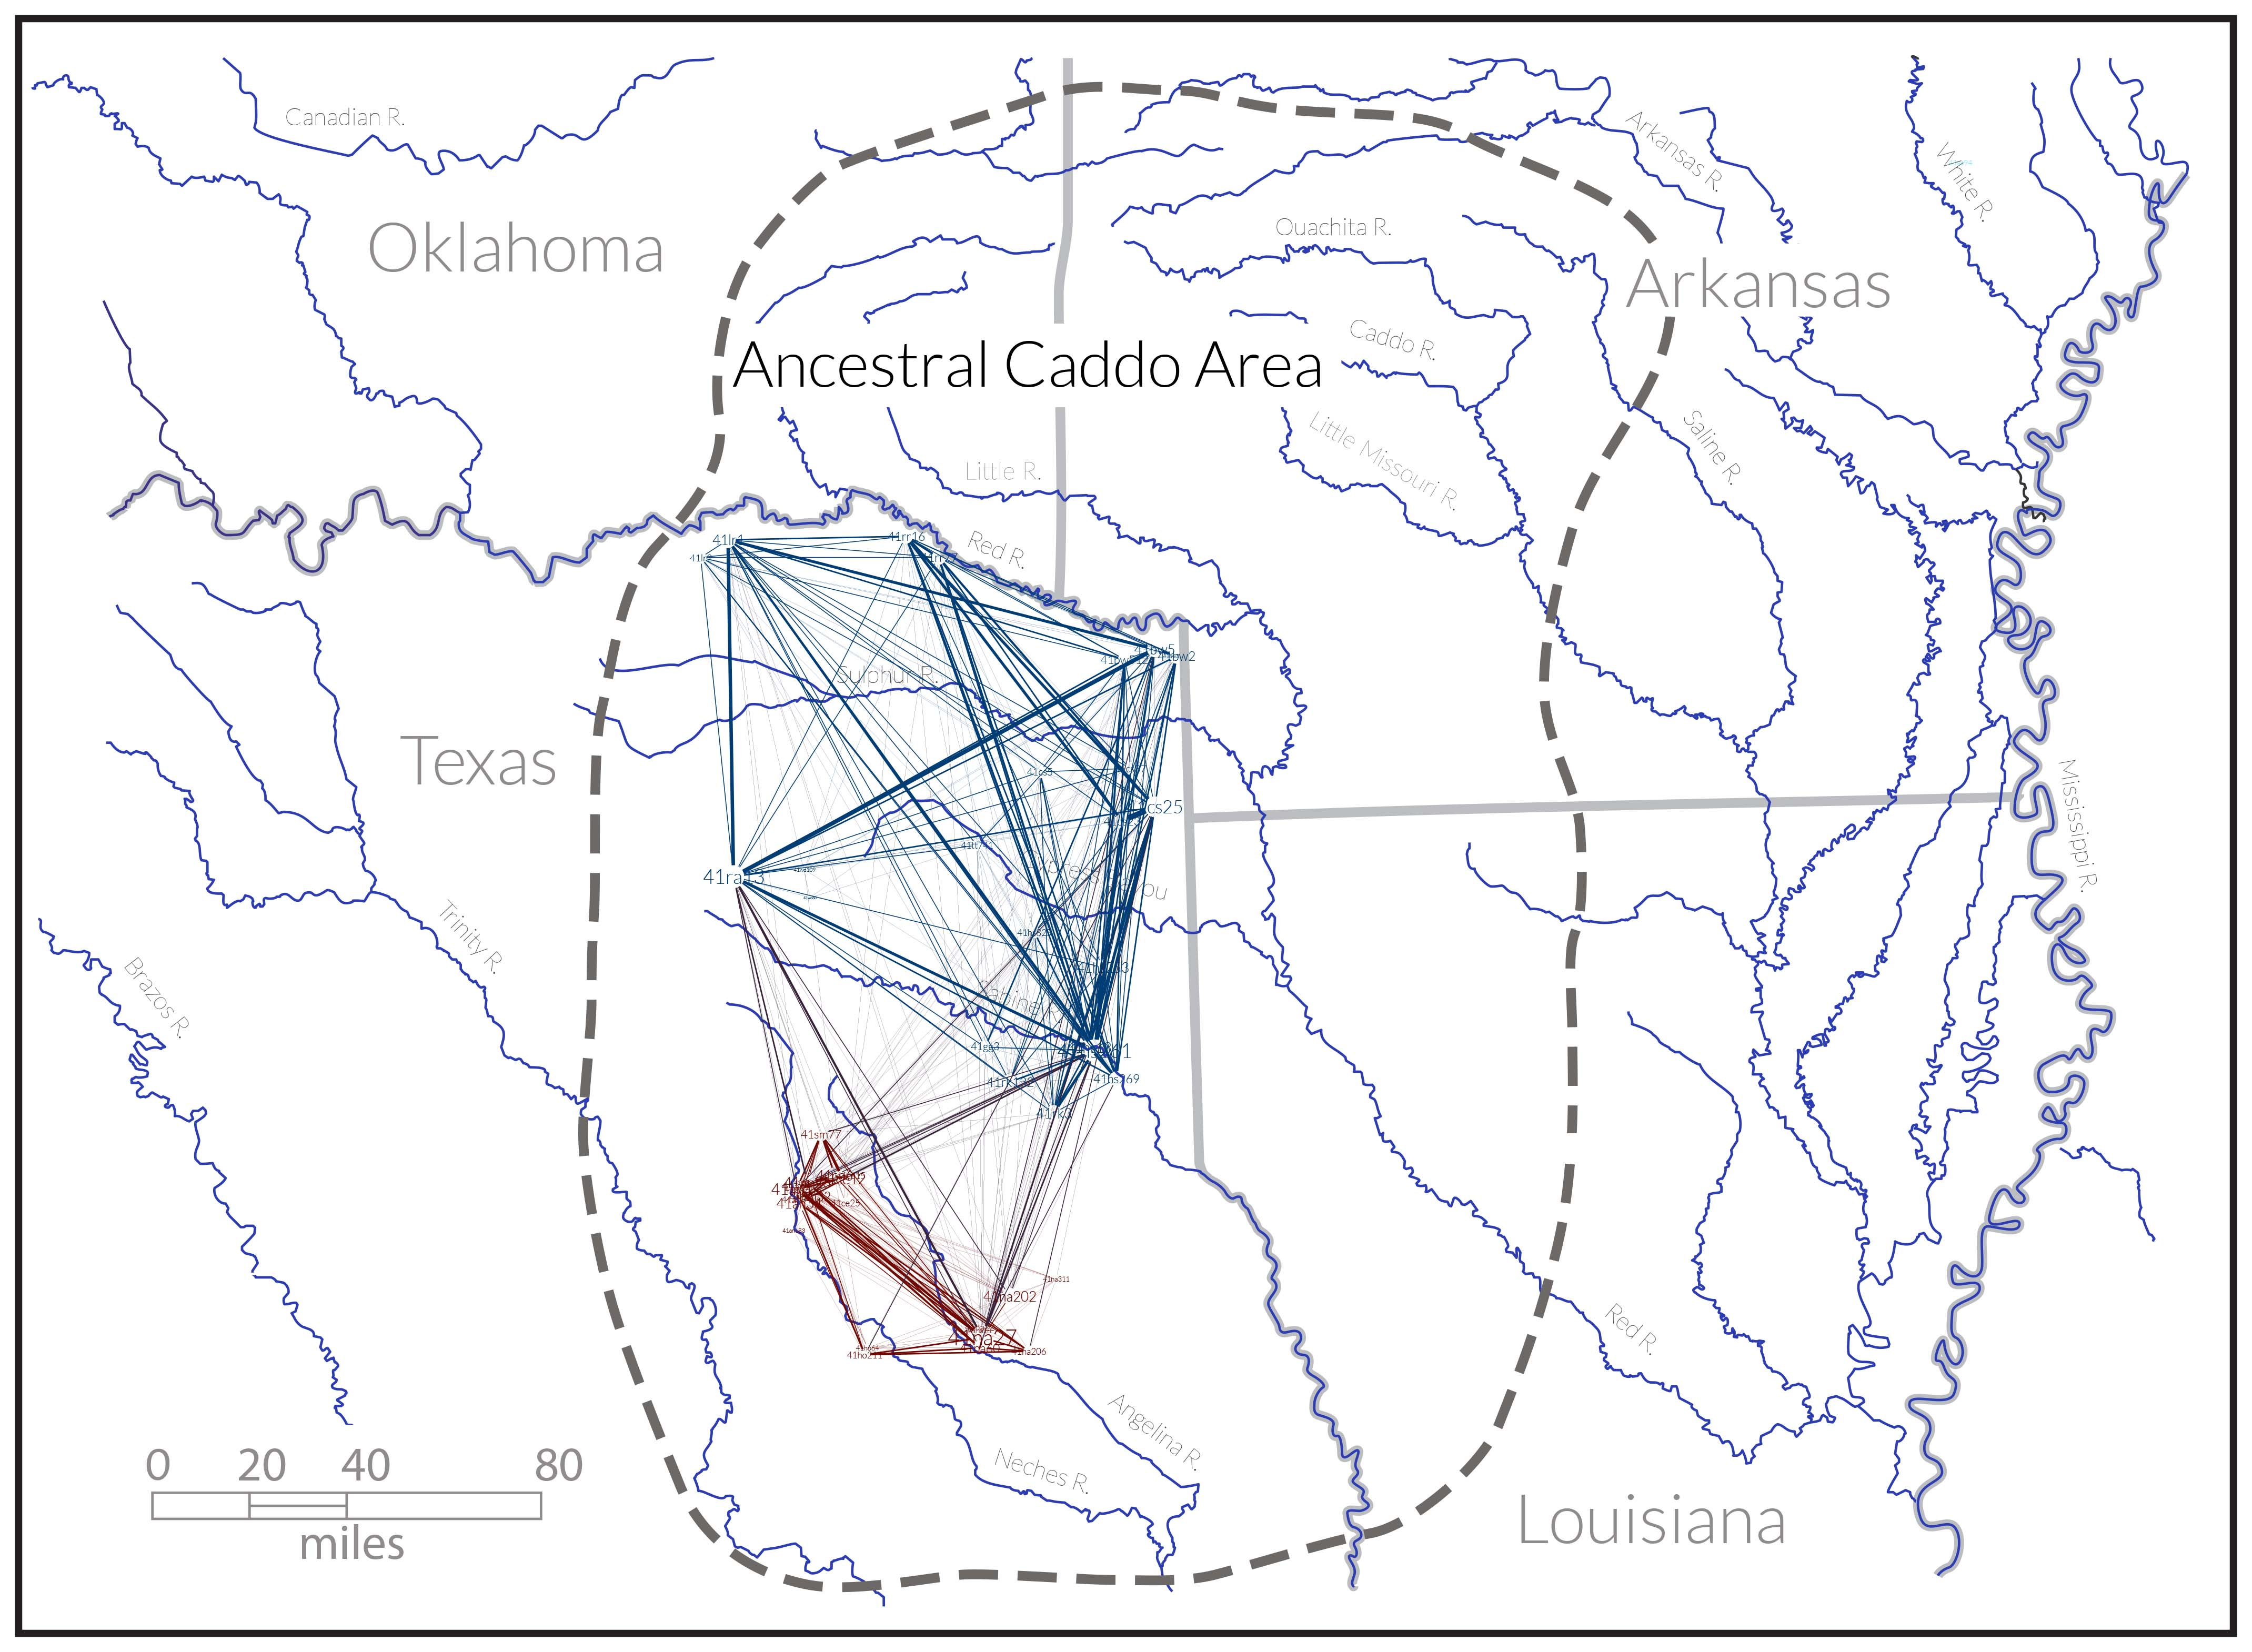
\includegraphics[width=1\linewidth]{ms-figs/figure1} \caption{Historic Caddo network generated using ceramic and lithic types, which include Perdiz arrow points (DOI 10.17605/OSF.IO/WD2ZT), illustrating the two (north [blue] and south [red]) Caddo behavioral regions. The regions were identified using a modularity statistic to secern those nodes more densely connected to one another than to the rest of the network.}\label{fig:fig1}
\end{figure}

The goal of this exploratory endeavor was to assess whether traditional
metrics collected for Perdiz arrow points support the \emph{shape
boundary} posited in recent social network and geometric morphometric
analyses, to determine whether linear metrics might be useful predictors
of regional membership, and---if so---to identify those morphological
features that articulate with each \emph{behavioral region} using
geometric morphometrics. It is assumed that complete Perdiz arrow points
included as offerings in Caddo burials represent the \emph{design
intent} of the maker. Should the analysis yield significant results, it
would bolster the argument for at least two discrete Caddo
\emph{behavioral regions} in northeast Texas; each empirically defined
by discernible morphological differences across three discrete
categories of Caddo material culture.

\hypertarget{caddo-behavioral-regions}{%
\subsection{\texorpdfstring{\emph{Caddo behavioral
regions}}{Caddo behavioral regions}}\label{caddo-behavioral-regions}}

In a June 18, 1937 Works Progress Administration interview with Lillian
Cassaway, Sadie Bedoka---a Caddo-Delaware woman raised with the
Caddo---stated that:

\begin{quote}
Each {[}Caddo{]} clan had its own shape to make its pottery. One clan
never thought of making anything the same pattern of another clan.
\emph{You could tell who made the pottery by the shape}
\cite[395]{RN9357x}.
\end{quote}

General differences in Caddo ceramic forms have been noted elsewhere
\cite{RN5650,RN7162}; however, the study of the Clarence H. Webb
collection was the first to illustrate a significant north-south
geographic shape difference among Hickory Engraved and Smithport Plain
Caddo bottle types \cite{RN8370}. That preliminary observation was later
confirmed using more robust samples of Hickory Engraved and Smithport
Plain bottles \cite{RN8074,RN7927}, then expanded to include a greater
variety of Caddo bottle types across a larger spatial and temporal
extent \cite{RN8312}.

The co-presence of diagnostic artifact and attribute types has been used
to define Caddo phases and periods, which serve as a heuristic tool that
aids archaeologists in explaining the local cultural landscape, as well
as regional differences between local landscapes. The Historic Caddo
network expands those efforts, augmenting the previously defined phases
and periods, and emphasizing the dynamic and manifold relational
connections that reinforce and transcend the currently-defined
categories \cite{RN8031}. This was achieved by enlisting a multi-scalar
methodological approach \cite{RN5644,RN8039}, where northern and
southern communities were parsed into constituent groups using the
co-presence of diagnostic types paired with a modularity statistic
\cite{RN8051,RN8024}. Most of the constituent groups identified in the
network analysis were found to articulate with known Caddo polities,
while others were not \cite{RN8031}.

A subsequent analysis of Gahagan bifaces confirmed that a second
category of Caddo material culture expressed significant morphological
differences across the same geography as the Hickory Engraved and
Smithport Plain bottles \cite{RN8158}. The morphology of Gahagan bifaces
from sites in central Texas was later found to differ significantly when
compared with those recovered from the Caddo region \cite{RN8322}. That
Gahagan bifaces were found to differ across two \emph{spatial
boundaries} was noteworthy, particularly since it has regularly been
assumed that these large bifaces were manufactured in central Texas and
arrived in the ancestral Caddo area as products of trade and/or exchange
\cite{RN8322,RN8158}. Further, that Gahagan bifaces were found to differ
across the same geography as those communities posited in the Historic
Caddo network analysis suggested that the temporal range of the
\emph{shape boundary} might extend to the Formative/Early Caddo period
(CE 800 - 1250); a hypothesis that was later confirmed in a more
comprehensive analysis of Caddo bottles \cite{RN8312}.

\hypertarget{methods-and-results}{%
\section{Methods and results}\label{methods-and-results}}

Sixty seven intact Perdiz arrow points recovered from Caddo burial
contexts in Camp, Nacogdoches, and Shelby counties comprise the basis of
this study (\href{https://seldenlab.github.io/perdiz3/}{supplementary
materials}). A standard suite of linear metrics were collected for each
specimen, including maximum length, width, thickness, stem length, and
stem width. Following collection, data were imported to R 4.1.1
\cite{RN8584} (\href{https://seldenlab.github.io/perdiz3/}{supplementary
materials}), where boxplots were produced, along with a Principal
Components Analysis (PCA) followed by analyses of variance (ANOVA) to
test whether the morphology of Perdiz arrow points differs across the
shape boundary (Fig.2).

Boxplots illustrate the distribution and mean for each of the five
variables (Fig. 2a-e), and the PCA (Fig. 2f) illustrates over 92 percent
of the variation in the sample among PC1 (84.65 percent) and PC2 (11.71
percent). ANOVAs demonstrate significant differences in Perdiz arrow
point morphology among four of the five variables (maximum length,
width, stem length, and stem width)
(\href{https://seldenlab.github.io/perdiz3/}{supplementary materials}).
Maximum thickness does not differ significantly between the northern and
southern communities, which led to the decision to conduct the
subsequent geometric morphometric analysis as a two dimensional, rather
than a three-dimensional, study
(\href{https://seldenlab.github.io/perdiz3/}{supplementary materials}).

\begin{figure}
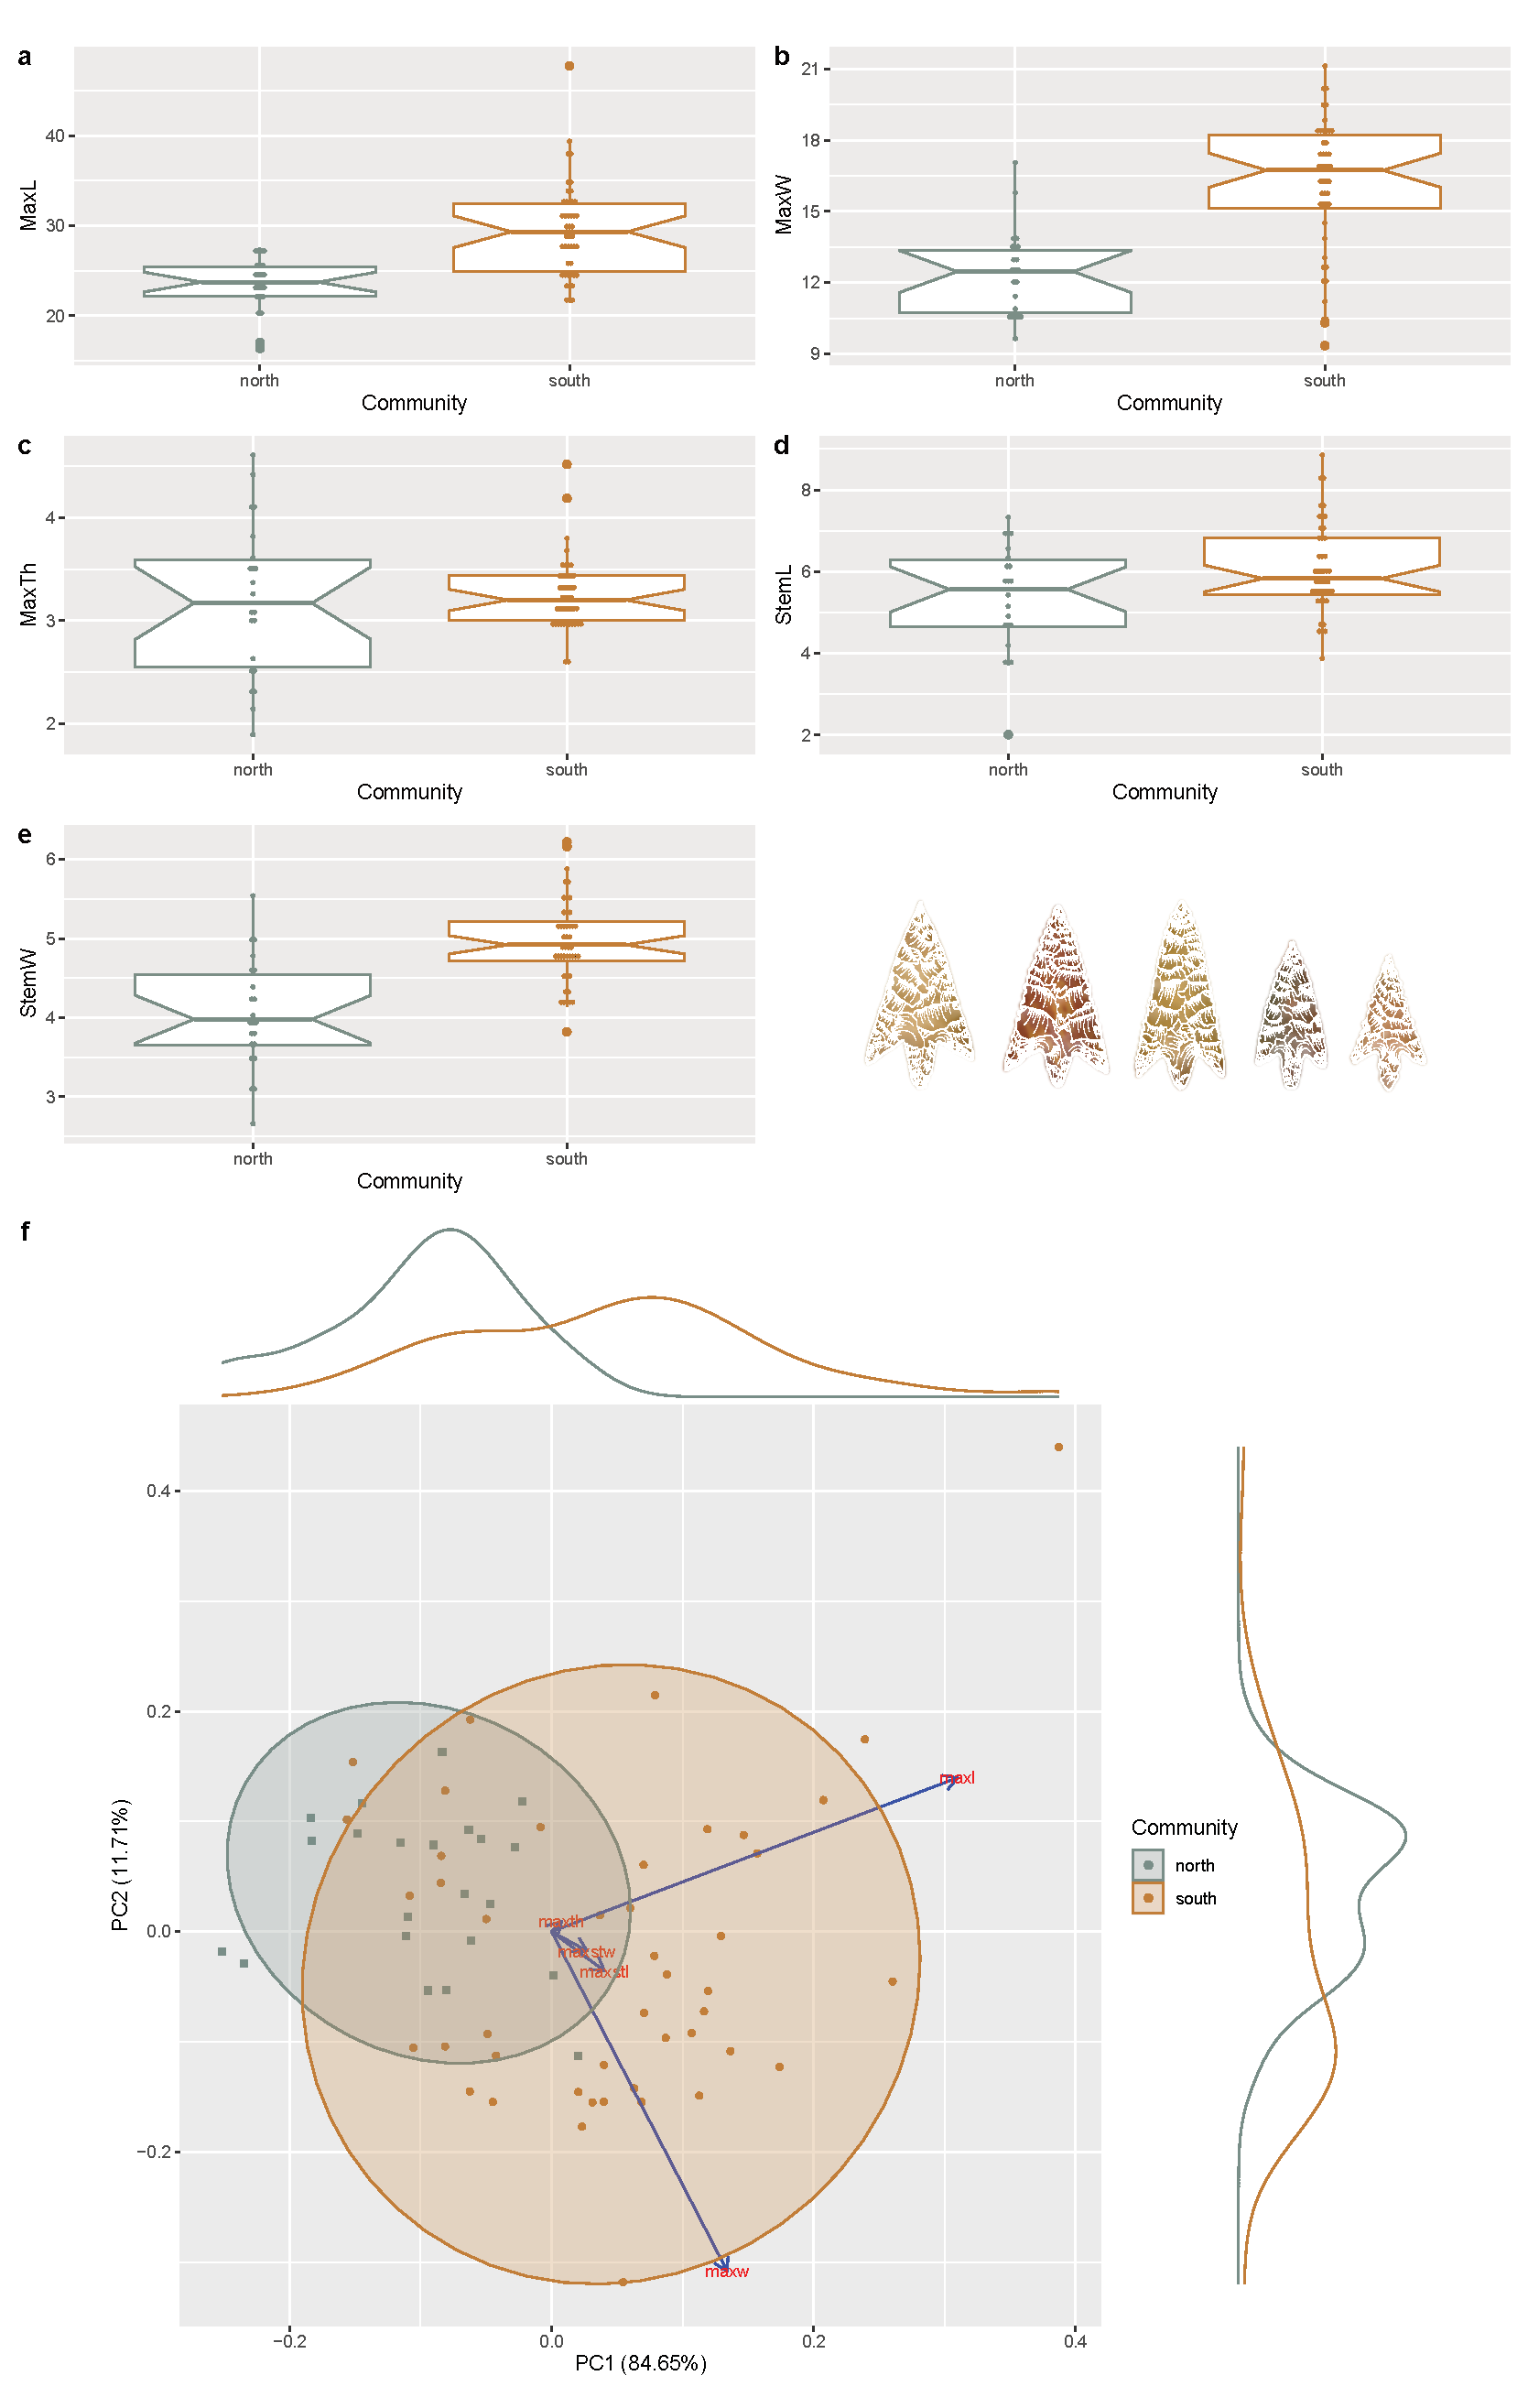
\includegraphics[width=0.95\linewidth]{ms-figs/figure2} \caption{Boxplots for a, maximum length; b, maximum width; c, maximum thickness; d, stem length; e, stem width, and f, PCA for linear metrics associated with the Perdiz arrow points. Additional information related to the analysis, including data and code needed to reproduce these results, can be found in the supplemental materials at https://seldenlab.github.io/perdiz3/.}\label{fig:fig2}
\end{figure}

\hypertarget{predictive-model}{%
\subsection{\texorpdfstring{\emph{Predictive
model}}{Predictive model}}\label{predictive-model}}

The utility of support vector machines to classify archaeological
materials has increased with the rise of big data and digital
repositories \cite{RN9515,RN9516,RN9514,RN9513}. For this effort, linear
data were imported and modeled using the \texttt{scikit-learn} package
in Python \cite{scikit-learn,sklearn_api}
(\href{https://seldenlab.github.io/perdiz3/}{supplementary materials}).
Data were subsequently split into training (75 percent) and testing (25
percent) subsets. A \emph{standard scaler} was used to decrease the
sensitivity of the algorithm to outliers by standardizing features, and
a \emph{nested cross validation} of the training set was used to achieve
unbiased estimates of model performance, resulting in a mean cross
validation score of 86 percent
(\href{https://seldenlab.github.io/perdiz3/}{supplementary materials}).
The model was subsequently fit on the training set, yielding a receiver
operator curve score of 97 percent, and an accuracy score of 94 percent
(\href{https://seldenlab.github.io/perdiz3/}{supplementary materials}).

\hypertarget{geometric-morphometrics}{%
\subsection{\texorpdfstring{\emph{Geometric
morphometrics}}{Geometric morphometrics}}\label{geometric-morphometrics}}

Each of the arrow points was imaged using a flatbed scanner (HP Scanjet
G4050) at 600 dpi. The landmarking protocol developed for this study
(\href{https://seldenlab.github.io/perdiz3/}{supplementary materials})
included six landmarks and 24 equidistant semilandmarks to characterize
Perdiz arrow point shape, applied using the \texttt{StereoMorph} package
in R \cite{RN8973}. The characteristic points and tangents used in the
landmarking protocol were inspired by the work of Birkhoff
\cite{RN5700}.

Landmarks were aligned to a global coordinate system
\cite{RN8102,RN8587,RN8384}, achieved through generalized Procrustes
superimposition \cite{RN8525} performed in R 4.1.1 \cite{RN8584} using
the \texttt{geomorph} package v4.0.0 \cite{RN8565}. Procrustes
superimposition translates, scales, and rotates the coordinate data
allowing for comparisons among objects \cite{RN5698,RN8525}. The
\texttt{geomorph} package uses a partial Procrustes superimposition that
projects the aligned specimens into tangent space subsequent to
alignment in preparation for the use of multivariate methods that assume
linear space \cite{RN8511,RN8384} (Fig.3).

\begin{figure}
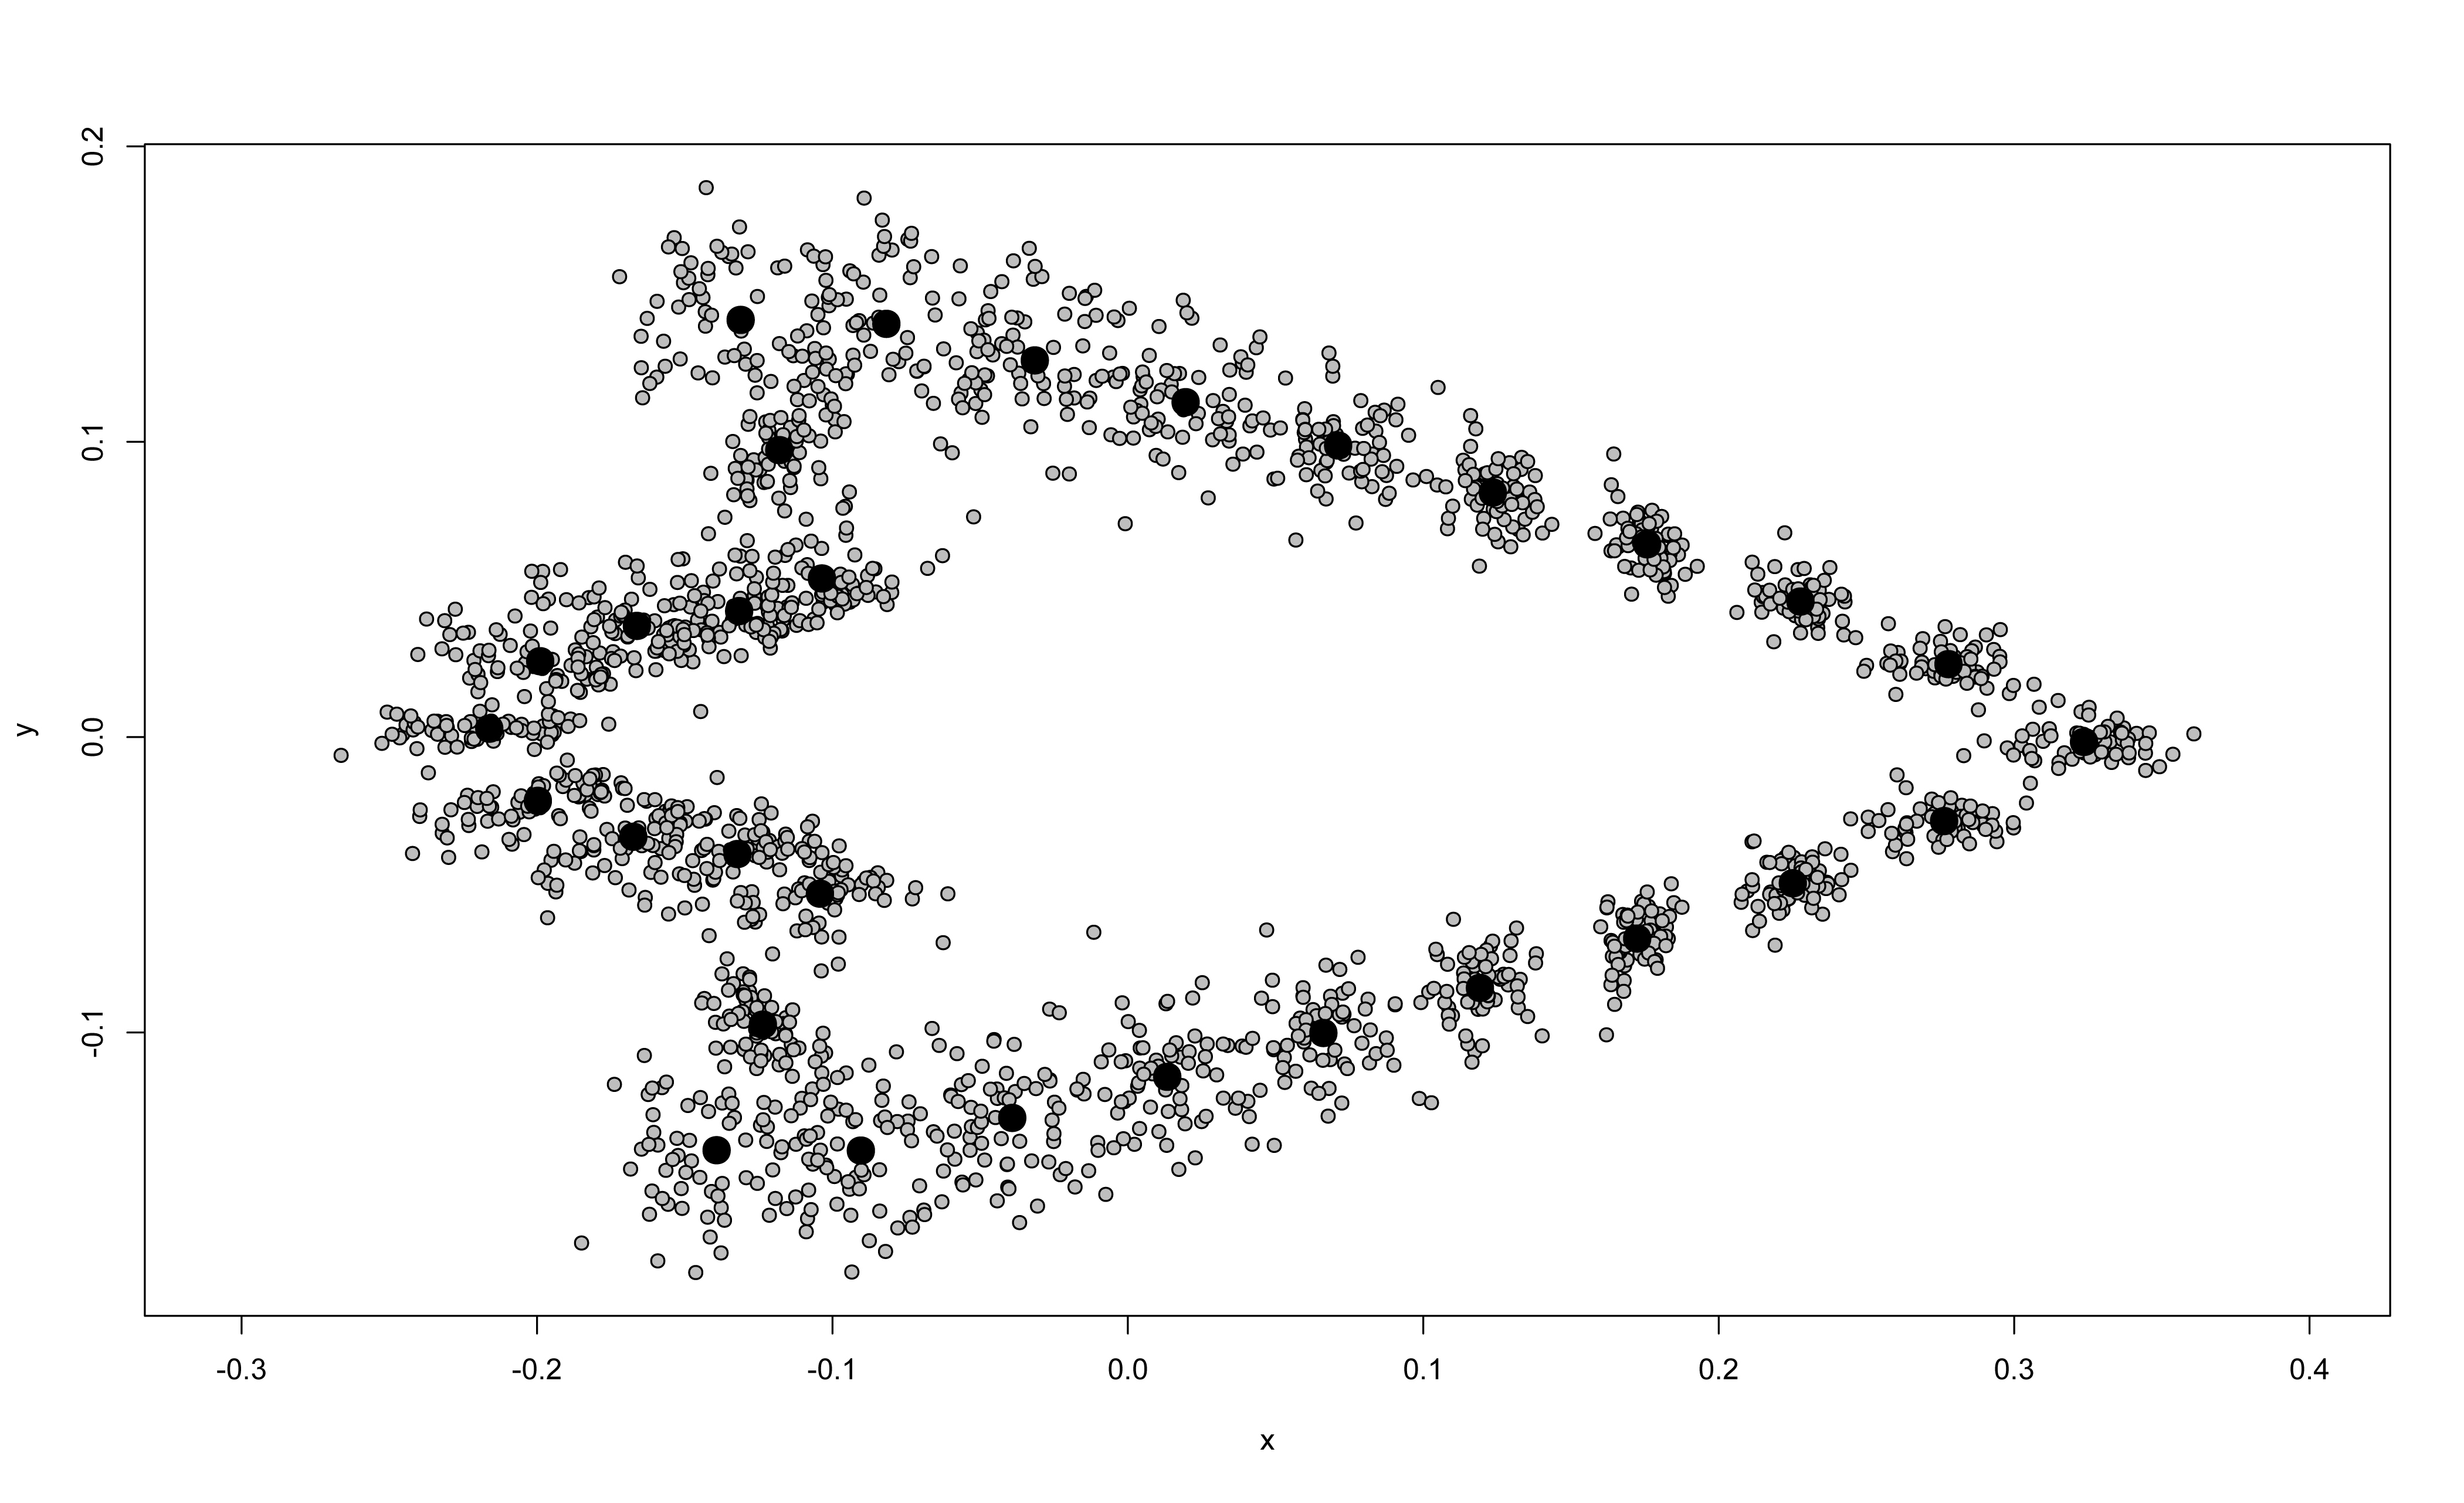
\includegraphics[width=1\linewidth]{ms-figs/figure3} \caption{Results of generalized Procrustes analysis, illustrating mean shape (black) and all specimens in the sample (gray). Additional information related to the GPA, including those data and code needed to reproduce these results, can be found in the supplemental materials at https://seldenlab.github.io/perdiz3/.}\label{fig:fig3}
\end{figure}

Principal components analysis \cite{RN8576} was used to visualize shape
variation among the arrow points (Fig. 4). The shape changes described
by each principal axis are commonly visualized using thin-plate spline
warping of a reference image or 3D mesh \cite{RN8555,RN8553}. A residual
randomization permutation procedure (RRPP; n = 10,000 permutations) was
used for all Procrustes ANOVAs \cite{RN8579,RN8334}, which has higher
statistical power and a greater ability to identify patterns in the data
should they be present \cite{RN6995}. To assess whether shape changes
with size (allometry), and differs by group (region), Procrustes ANOVAs
\cite{RN7046} were also run that enlist effect-sizes (z-scores) computed
as standard deviates of the generated sampling distributions
\cite{RN8477}. Procrustes variance was used to discriminate between
regions and compare the amount of shape variation (morphological
disparity) \cite{RN5703}, estimated as the Procrustes variance using
residuals of linear model fit \cite{RN8314}. A pairwise comparison of
morphological integration was used to test the strength of integration
between blade and basal morphology using a z-score \cite{RN8340}.

\begin{figure}
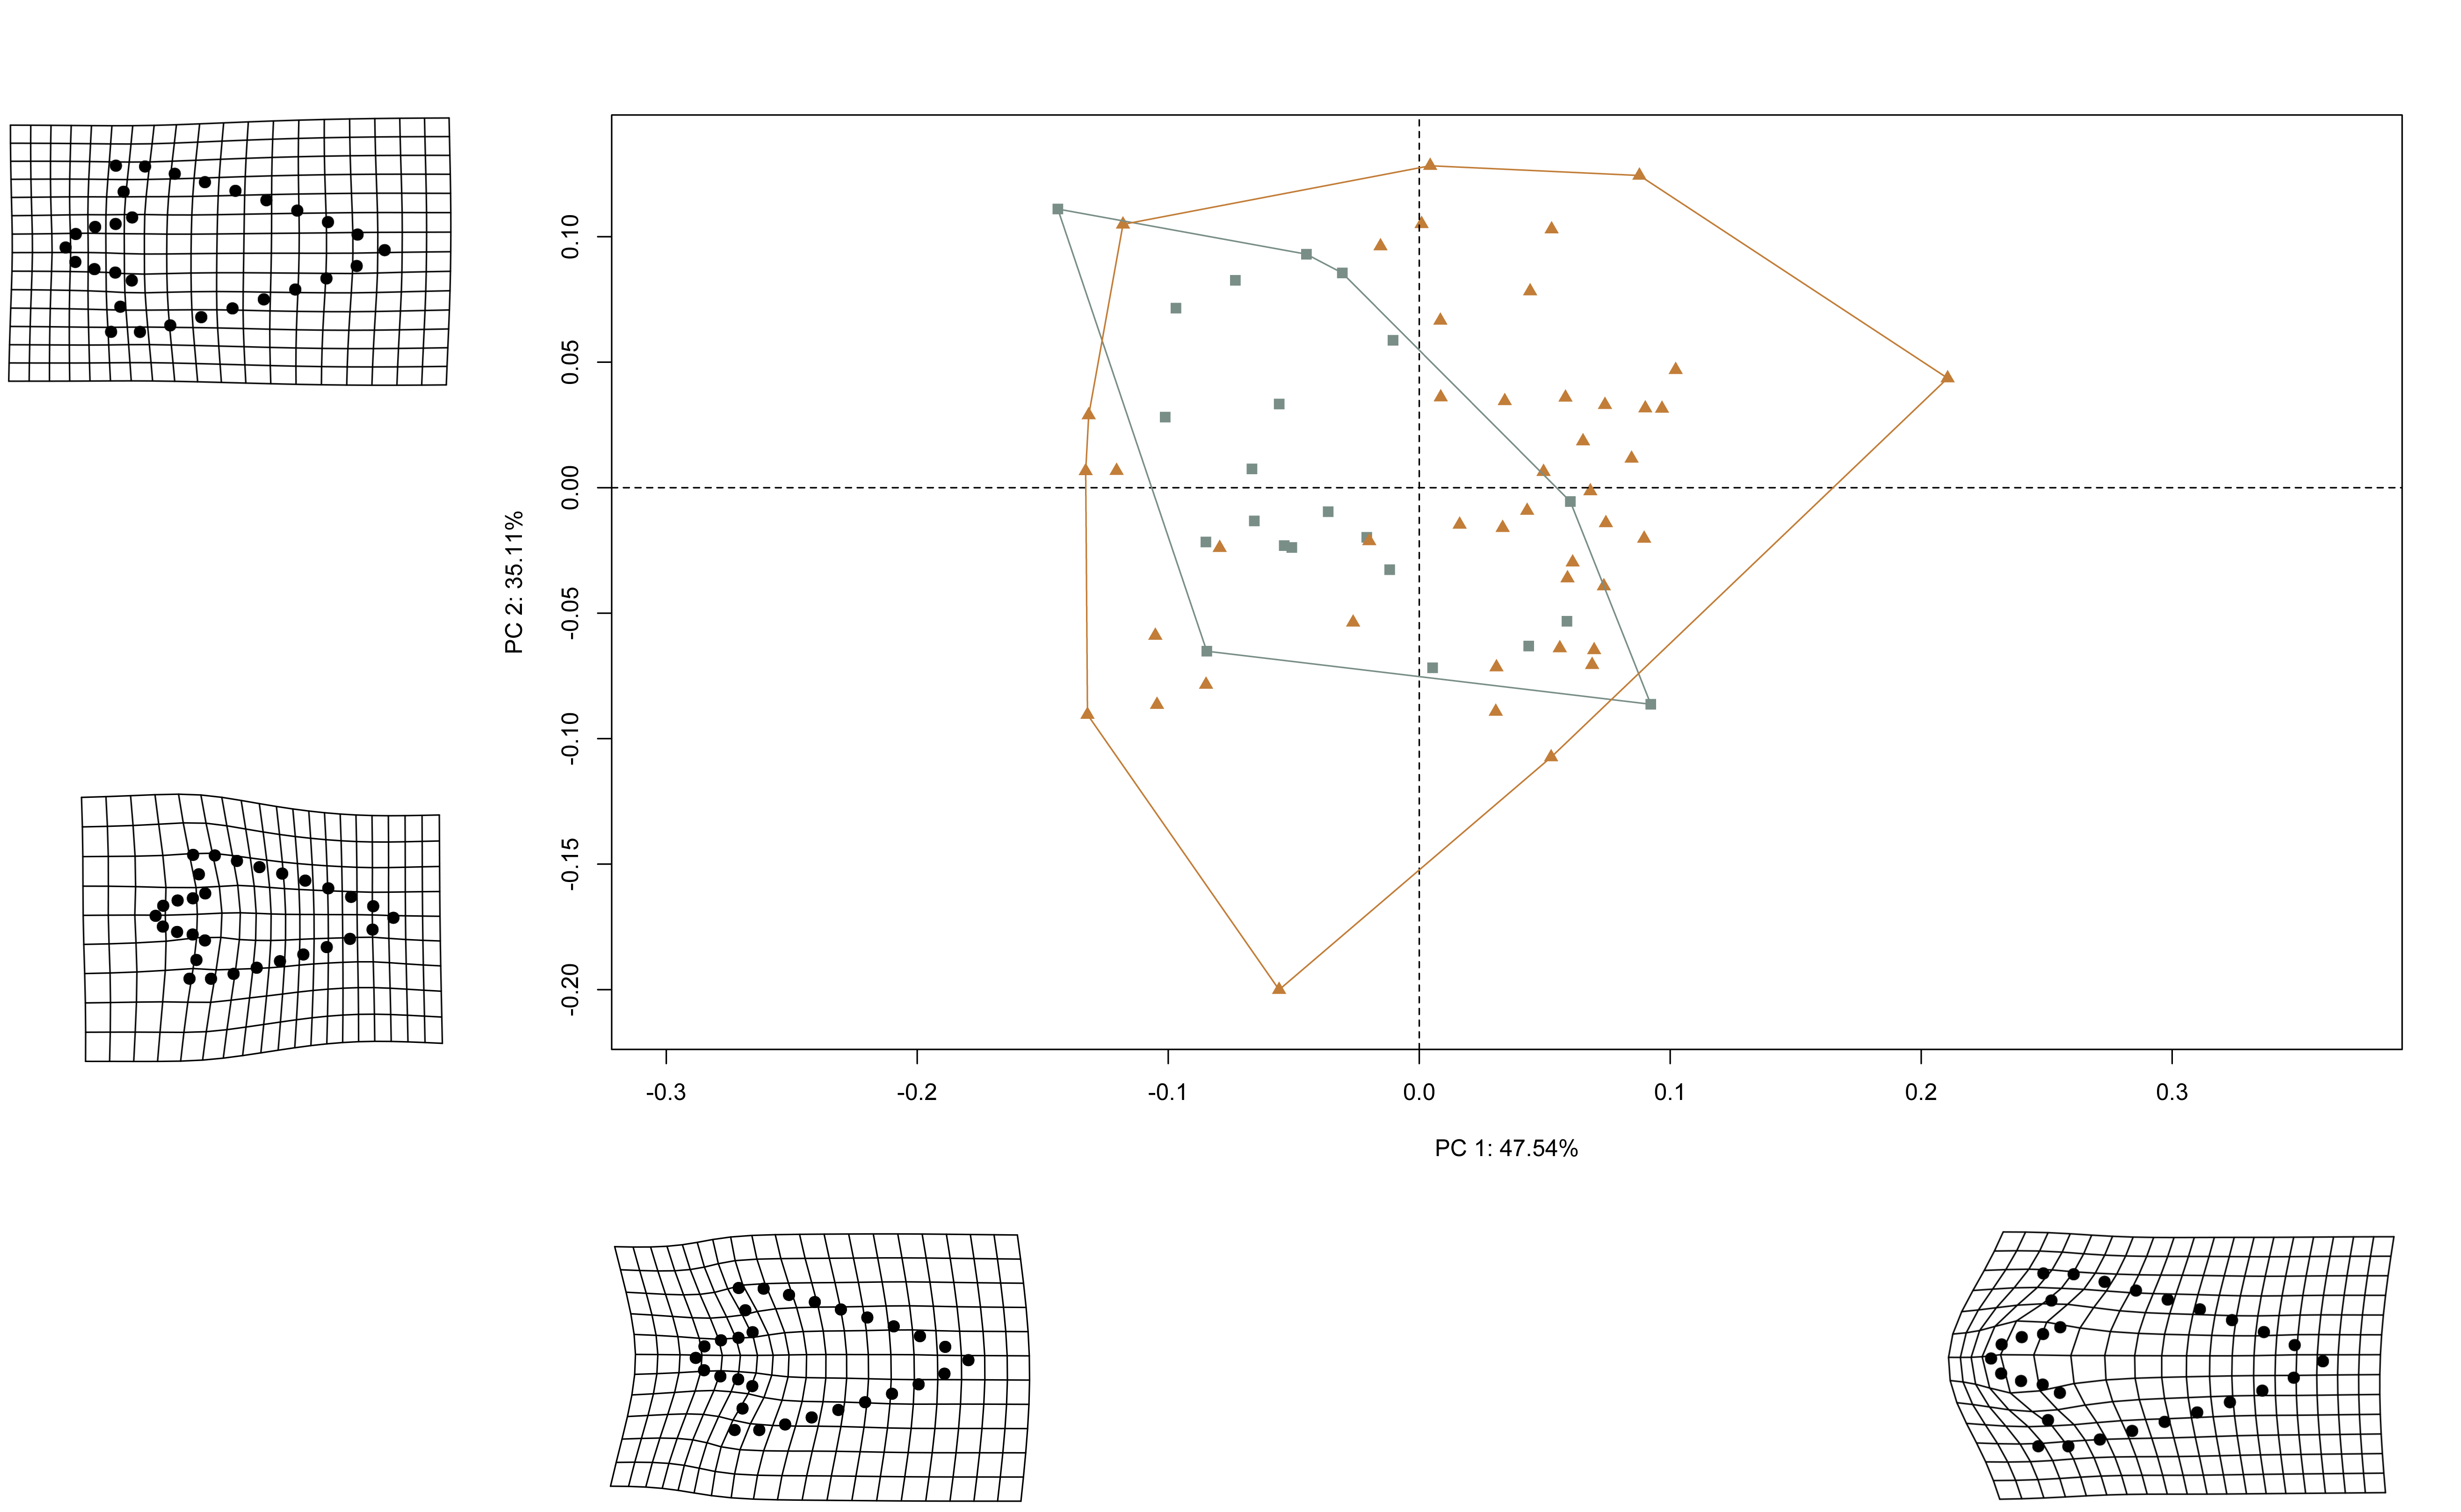
\includegraphics[width=1\linewidth]{ms-figs/figure4} \caption{Principal components analysis plot (PC1/PC2) for Perdiz arrow points by behavioral region/community (top; gray squares, north; orange triangles, south), and results of modularity (bottom left) and blade/base morphological integration (bottom right) analyses. Additional information related to the PCA, including the full listing of results and those data and code needed to reproduce these results, can be found in the supplemental materials at https://seldenlab.github.io/perdiz3/.}\label{fig:fig4}
\end{figure}

The analysis of modularity, which compares within-module covariation of
landmarks against between-module covariation was significant (Fig. 4 and
\href{https://seldenlab.github.io/perdiz3/}{supplementary materials}),
demonstrated that Perdiz arrow point blades and bases are, in fact,
modular. The test for morphological integration was also significant
(Fig. 4 and \href{https://seldenlab.github.io/perdiz3/}{supplementary
materials}), indicating that the blades and bases of Perdiz arrow points
are integrated. These results demonstrate that blade and base shapes for
Perdiz arrow points are predictable; a finding that would have great
utility in studies of Perdiz arrow point morphology that incorporate
fragmentary specimens.

A Procrustes ANOVA was used to test whether a significant difference
exists in Perdiz arrow point (centroid) size (RRPP = 10,000; Rsq =
0.30681; Pr(\textgreater F) = 1e-04), followed by a second to test
whether a significant difference exists in arrow point shape by region
(northern vs.~southern communities) (RRPP = 10,000; Rsq = 0.0536;
Pr(\textgreater F) = 0.0161). A comparison of mean consensus
configurations was used to characterize intraspecific shape variation of
Perdiz arrow points from the northern and southern \emph{behavioral
regions}. Diacritical morphology occurs primarily in basal shape, where
the angle between the shoulder and base is more acute, and a base that
is generally shorter and narrower in the southern \emph{behavioral
region} than it is in the north (Fig. 5 and
\href{https://seldenlab.github.io/perdiz3/}{supplementary materials}).

\begin{figure}
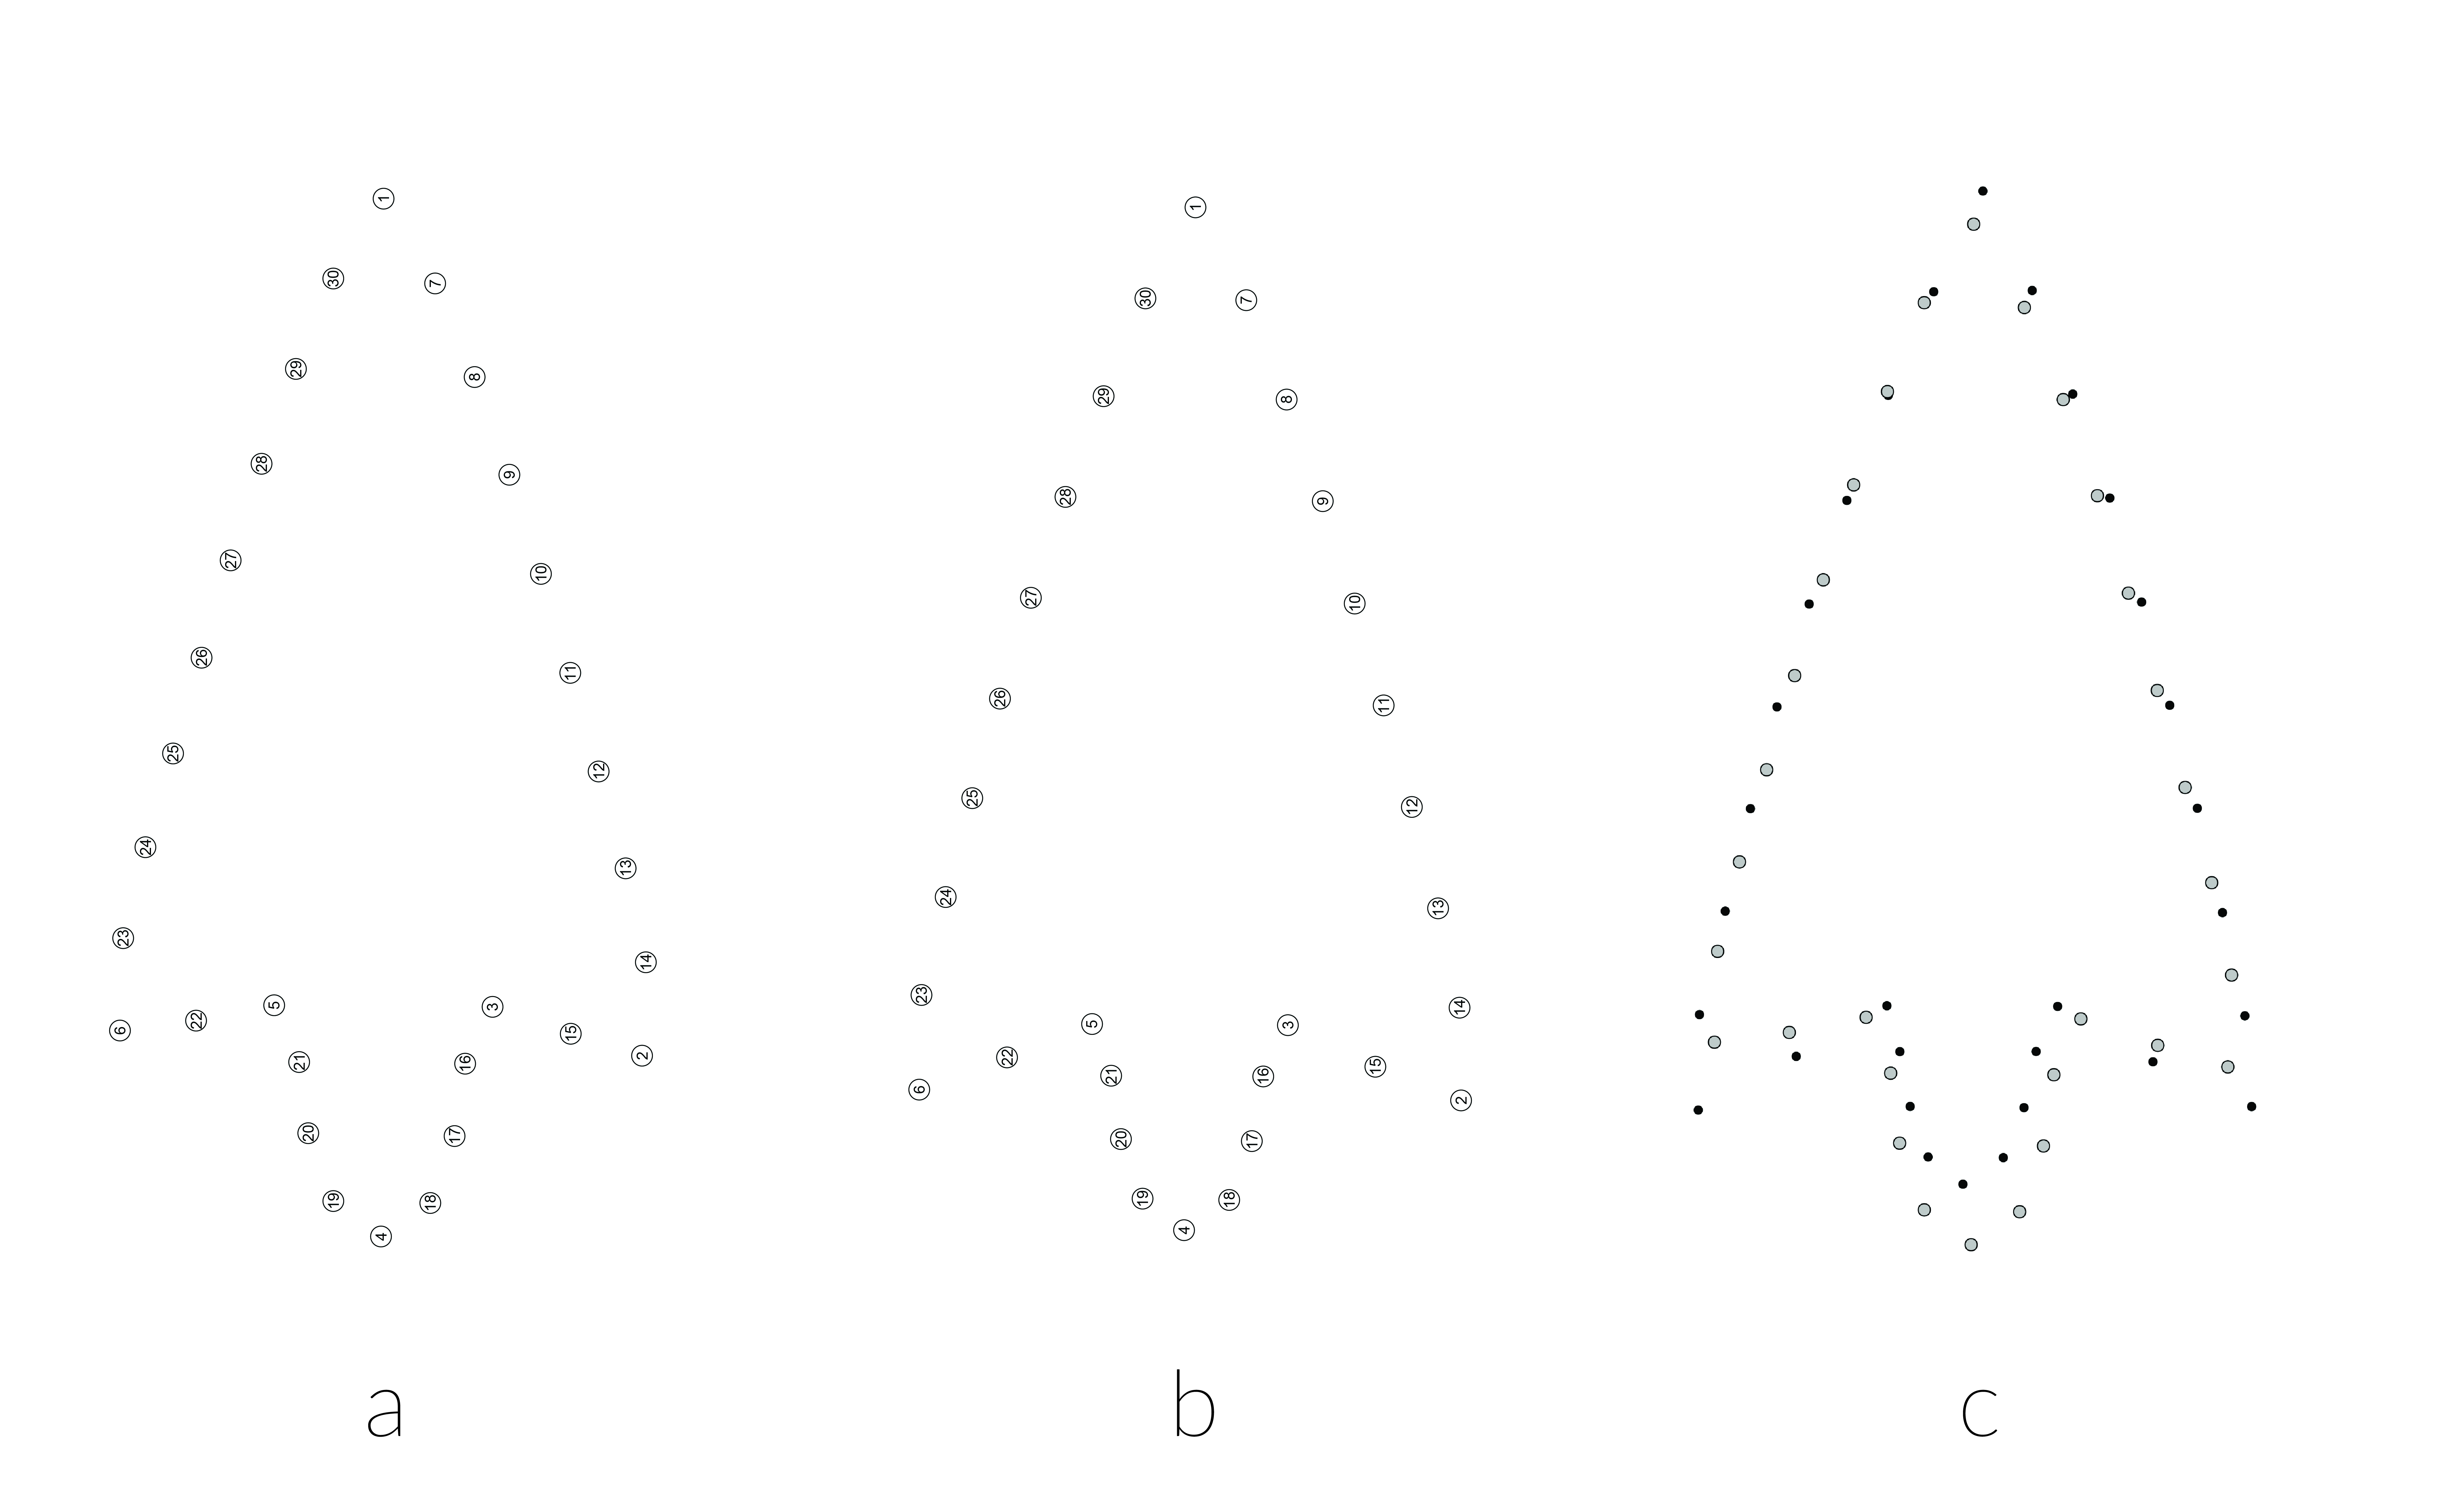
\includegraphics[width=1\linewidth]{ms-figs/figure5} \caption{Mean shapes for Perdiz arrow points from the northern (left), and southern (center) behavioral region. In the comparison of the two (right), the northern behavioral region is represented by gray circles, and the southern, by black. Additional information related to the mean shapes, including those data and code needed to reproduce these results, can be found in the supplemental materials at https://seldenlab.github.io/perdiz3/.}\label{fig:fig5}
\end{figure}

\hypertarget{discussion}{%
\section{Discussion}\label{discussion}}

The \emph{shape boundary} empirically delineates two discrete
\emph{behavioral regions} in the ancestral Caddo area. That the Perdiz
arrow points recovered from Caddo burials north and south of the
\emph{shape boundary} were found to differ significantly, expands the
scope of the \emph{behavioral regions} to include three classes of
artifacts (Caddo bottles, bifaces, and---now---arrow points)
\cite{RN8074,RN7927,RN8370,RN8312,RN8322,RN8158}. Results clearly
illustrate that those morphological differences among Perdiz arrow
points found in the northern and southern \emph{behavioral regions} are
predictable (\href{https://seldenlab.github.io/perdiz3/}{supplementary
materials}), and can be disaggregated using the standard suite of linear
metrics regularly collected in the context of cultural resource
management endeavors.

The geometric morphometric analysis demonstrated significant
morphological differences for Perdiz arrow points recovered north and
south of the \emph{shape boundary}, where the most pronounced difference
was found to occur in basal morphology (see Fig. 5). Allometry was also
found to be significant, demonstrating that the shape of Perdiz arrow
points differs with size. Those arrow points used in this study are
considered to represent \emph{design intent}, and are not thought to
exhibit retouch or resharpening. This finding provides evidence in
support of the argument that Perdiz arrow point morphology is labile
\cite{RN9364}.

Blades and bases of Perdiz arrow points were found to be both modular
and morphologically integrated. This indicates that each module
functions independently, and that base shape is a predictor of blade
shape, and vice-versa. Further work is warranted to assess whether
Perdiz arrow points from groups within the boundaries of the northern
and southern \emph{behavioral regions} may express unique morphologies,
aiding in further delimiting local boundaries associated with
constituent Caddo groups. Whether, and to what extent, it may be
possible to identify specific groups of makers using unmodified arrow
points from Caddo mortuary contexts remains unknown. Additional
complexity is introduced when considering that Perdiz arrow points
included in Caddo burials may have been manufactured elsewhere then
transported to the ancestral Caddo territory, where they were
potentially placed in burials by members of non-Caddo groups. This
challenges the concept that all cultural material recovered from Caddo
burials was manufactured by, and placed with the deceased, only by
members of a specific Caddo family, group, or polity.

\hypertarget{standardization-andor-specialization}{%
\subsection{\texorpdfstring{\emph{Standardization and/or
specialization}}{Standardization and/or specialization}}\label{standardization-andor-specialization}}

Morphological attributes are representative of intentional attributes
related to morphological characteristics \cite{RN7051}, and dimensional
standardization has utility in identifying the range of variation and
overlap of product morphology both in and between communities
\cite{RN5779}. Further, relative dimensional standardization may imply a
smaller number of production units contrasted with larger production
units \cite{RN7051}.

While the Caddo bottles are representative of a complete system---or
unit---the function of a biface (Perdiz arrow points and Gahagan bifaces
in this context) is more limited, in that they represent only a single
component of a much more dynamic system. Dimensional standardization in
size has been identified for both the Caddo bottles and Gahagan bifaces.
The similarities and differences in bottle shapes were found to
transcend typological assignments, and bottles from the northern
\emph{behavioral region} were found to express a significantly greater
diversity in size, yielding evidence for size standardization in the
southern \emph{behavioral region}. It is also the case that Gahagan
bifaces from the Caddo area were found to express a significantly
greater diversity in size compared to those from central Texas. These
findings suggest that there may have been local limits on the social
tolerance for specific technological or aesthetically acceptable
morphological traits.

\hypertarget{morphologically-distinct-behavioral-regions}{%
\subsection{\texorpdfstring{\emph{Morphologically-distinct behavioral
regions}}{Morphologically-distinct behavioral regions}}\label{morphologically-distinct-behavioral-regions}}

In considering the role(s) of artifacts as aspects of \emph{social
identity}, it is important not to lose sight of the fact that people and
artifacts are active agents in the production and maintenance of
\emph{social identity(ies)}. Both categories of artifacts (bottles and
bifaces) contribute to local and regional \emph{communities of identity}
and \emph{communities of practice} \cite{RN8061}. Generally, this
concept may be more easily applied to bottles since they were
manufactured and used by individuals sharing collective \emph{Caddo
identities}. Bifaces (Perdiz arrow points and Gahagan bifaces)
potentially represent multiple \emph{identities}---those being the
Caddo, as users; and non-Caddo, as producers---at least with regard to
chipped stone tools incorporated in mortuary contexts. This idea lends
defensible credence to the concept of morphologically-distinct
\emph{behavioral regions} among the Caddo, while integrating the
possibility of understanding interactions between Caddo and non-Caddo
groups, to include the movement of material culture between Caddo
\emph{behavioral regions}.

Three categories of Caddo material culture differ north and south of the
\emph{shape boundary}, indicate a haecceity of regionally-distinct
perspectives related to production (bottles), and/or aesthetic
choice/cultural interaction (bifaces). These differing perspectives
incorporate group decisions that include shape, size, form, and
decorative expression, which likely represent the culmination of
generational perspectives \cite{RN5610}. Simply stated, such
perspectives are representative of tradition. Eckert and colleagues
\cite{RN8061} indicate that provenance, the origin or source of an item,
is a significant component of understanding the interrelatedness of
\emph{communities of identity} and \emph{communities of practice}.
Perdiz arrow points and Gahagan bifaces recovered north and south of the
\emph{shape boundary} are morphologically distinct. A second \emph{shape
boundary} demonstrates that Gahagan bifaces differ significantly between
the ancestral Caddo region and central Texas, where they are currently
thought to have been manufactured. This suggests that those
\emph{communities of practice} that articulate with the production of
chipped stone artifacts recovered from Caddo internments, are not Caddo.

It is entirely possible that there are no \emph{communities of practice}
at all for chipped stone artifacts recovered from Caddo mortuary
contexts. However, there do appear to have been \emph{communities of
practice} associated with Perdiz arrow points recovered from
non-mortuary contexts in the ancestral Caddo area, which may more
readily reflect the distinct retouch or resharpening approaches employed
by Caddo knappers \cite{RN9364}. Similar interpretations can be applied
to Gahagan bifaces, as few have been reported outside of Caddo mortuary
contexts. It may be more fitting to perceive of Perdiz arrow points and
Gahagan bifaces as indicative of \emph{communities of identity} rather
than \emph{communities of practice}, due to the contextual discrepancy
evinced through mortuary and non-mortuary settings. The provenance of
bifaces from Caddo mortuary contexts can most assuredly be considered
non-local, or produced outside of the ancestral Caddo region, based on
multiple factors that include raw material, workmanship, morphology, and
context.

\hypertarget{conclusion}{%
\section{Conclusion}\label{conclusion}}

This exploratory study demonstrated that linear metrics collected for
Perdiz arrow points support the \emph{shape boundary} posited in recent
social network and geometric morphometric analyses, and determined that
the same metrics can be used to predict regional membership. Those
morphological features that discriminate between Perdiz arrow points
recovered from each \emph{behavioral region} were identified using
geometric morphometrics, with the most substantial differences found to
occur in size and basal morphology. Blade and base shape were found to
be both modular and morphologically integrated, suggesting that blade
and base shapes are predictable. While evidence from one
category---Caddo bottles---supports discussions of Caddo production, the
other two---bifaces---more readily articulate with production activities
outside of the region by non-Caddo makers. Such production activity is
more likely to be localized than exchange systems, thus assumed to leave
a clearer signature \cite{RN7019}. Further work is warranted to expand
the scope of this research program to include analyses of differential
production within the two \emph{behavioral regions} outlined in this
study using a greater diversity of diagnostic Caddo artifact types.

\hypertarget{acknowledgments}{%
\section*{Acknowledgments}\label{acknowledgments}}
\addcontentsline{toc}{section}{Acknowledgments}

We express our gratitude to the Caddo Nation of Oklahoma and the
Anthropology and Archaeology Laboratory at Stephen F. Austin State
University for the requisite permissions and access to the NAGPRA
objects from the Washington Square Mound site and Turner collections,
and to Tom A. Middlebrook for brokering access to the Perdiz arrow
points from burials at the Morse Mound site. Thanks also to the editors,
contributors, and reviewers for their useful comments and constructive
criticisms, which further improved this manuscript.

\hypertarget{data-management}{%
\section*{Data Management}\label{data-management}}
\addcontentsline{toc}{section}{Data Management}

The data and analysis code associated with this project can be accessed
through the GitHub repository
(\url{https://github.com/seldenlab/perdiz3}) or the supplementary
materials (\url{https://seldenlab.github.io/perdiz3/}); which are
digitally curated on the Open Science Framework at \newline DOI:
10.17605/OSF.IO/UK9ZD.


\bibliographystyle{spphys}
\bibliography{mybibfile.bib}

\end{document}
